118.\begin{figure}[ht!]
\center{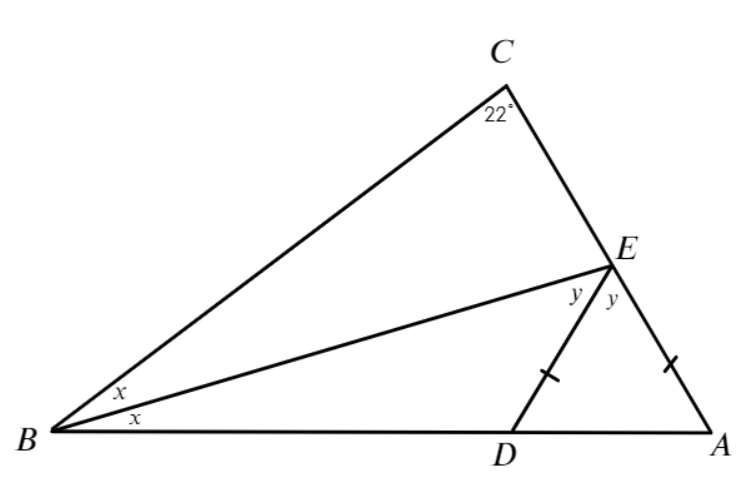
\includegraphics[scale=0.35]{g118.png}}
\end{figure}\\
Обозначим $\angle CBE=\angle EBD=x,\ \angle BED=\angle DEA=y.$ Тогда $\angle BEC=180^\circ-2y$ и из треугольника $BCE:\ x+22^\circ+180^\circ-2y=180^\circ,\ 2y-x=22^\circ.$ Треугольник $EDA$ является равнобедренным, поэтому $\angle A=(180^\circ-y):2=90^\circ-\frac{1}{2}y.$ Тогда из треугольника $ABC:\ 2x+22^\circ+90^\circ-\frac{1}{2}y=180^\circ,\ 2x-\frac{1}{2}y=68^\circ.$ Домножим второе полученное равенство на 4 и сложим с первым: $2y-x+8x-2y=22^\circ+272^\circ,\ 7x=294^\circ,\ x=42^\circ.$ Значит, $\angle ABC=2\cdot42^\circ=84^\circ.$\\
